\documentclass{ximera}

\begin{document}
\begin{problem}
  For a certain vector-valued function $\vec{r}$, someone has plotted the derivative $\vec{r}'$ below:
  \begin{image}
    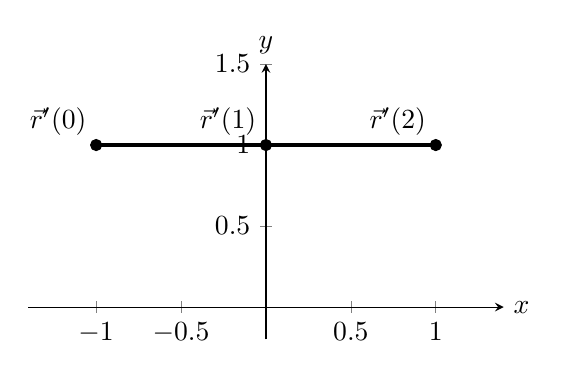
\begin{tikzpicture}
      \begin{axis}[
          xmin=-1.4, xmax=1.4, ymin =-.2, ymax =1.5,
          axis lines=center,
          width=3in,
          height=2in,
          xlabel=$x$,  
          ylabel=$y$,  
          every axis y label/.style={at=(current axis.above origin),anchor=south},  
          every axis x label/.style={at=(current axis.right of origin),anchor=west}
        ]
        \node[above left,black] at (axis cs: -1,1) {$\vec{r}'(0)$};
        \node[above left,black] at (axis cs: 0,1) {$\vec{r}'(1)$};
        \node[above left,black] at (axis cs: 1,1) {$\vec{r}'(2)$};
                
        \addplot[color=black,ultra thick] coordinates {(-1,1) (1,1)};
        \addplot[color=black,fill=black,only marks,mark=*] coordinates{(-1,1)};
        \addplot[color=black,fill=black,only marks,mark=*] coordinates{(0,1)};
        \addplot[color=black,fill=black,only marks,mark=*] coordinates{(1,1)};
        
      \end{axis}
    \end{tikzpicture}
  \end{image}
  If $\vec{r}(0) = \vector{-1,-1}$, which plot below represents
  $\vec{r}$? \pdfOnly{\textbf{Circle one.}}
\pdfOnly{\begin{center}
  \resizebox{1.4in}{!}{\begin{tikzpicture}
      \begin{axis}[
          xmin=-2, xmax=2, ymin =-2, ymax = 2,
          axis lines=center,  
          xlabel=$x$,  
          ylabel=$y$,  
          every axis y label/.style={at=(current axis.above origin),anchor=south},  
          every axis x label/.style={at=(current axis.right of origin),anchor=west}
        ]
        \addplot [black,ultra thick,domain=0:2,smooth] ({x^2/2-x-1},{x-1});
      \end{axis}
    \end{tikzpicture}}\quad
    \resizebox{1.4in}{!}{\begin{tikzpicture}
      \begin{axis}[
          xmin=-2, xmax=2, ymin =-2, ymax = 2,
          axis lines=center,  
          xlabel=$x$,  
          ylabel=$y$,  
          every axis y label/.style={at=(current axis.above origin),anchor=south},  
          every axis x label/.style={at=(current axis.right of origin),anchor=west}
        ]
        \addplot [black,ultra thick,domain=0:2,smooth] ({x-1},{x-1});
      \end{axis}
    \end{tikzpicture}}\quad
    \resizebox{1.4in}{!}{\begin{tikzpicture}
      \begin{axis}[
          xmin=-2, xmax=2, ymin =-2, ymax = 2,
          axis lines=center,  
          xlabel=$x$,  
          ylabel=$y$,  
          every axis y label/.style={at=(current axis.above origin),anchor=south},  
          every axis x label/.style={at=(current axis.right of origin),anchor=west}
        ]
        \addplot [black,ultra thick,domain=0:2,smooth] ({-1+x},{-1});
      \end{axis}
    \end{tikzpicture}}\quad
    \resizebox{1.4in}{!}{\begin{tikzpicture}
      \begin{axis}[
          xmin=-2, xmax=2, ymin =-2, ymax = 2,
          axis lines=center,  
          xlabel=$x$,  
          ylabel=$y$,  
          every axis y label/.style={at=(current axis.above origin),anchor=south},  
          every axis x label/.style={at=(current axis.right of origin),anchor=west}
        ]
        \addplot [black,ultra thick,domain=0:2,smooth] ({x^2/2-1},{x-1});
      \end{axis}
    \end{tikzpicture}}
\end{center}}
\begin{onlineOnly}
  \begin{multipleChoice}
    \choice[correct]{\resizebox{1.4in}{!}{\begin{tikzpicture}
      \begin{axis}[
          xmin=-2, xmax=2, ymin =-2, ymax = 2,
          axis lines=center,  
          xlabel=$x$,  
          ylabel=$y$,  
          every axis y label/.style={at=(current axis.above origin),anchor=south},  
          every axis x label/.style={at=(current axis.right of origin),anchor=west}
        ]
        \addplot [black,ultra thick,domain=0:2,smooth] ({x^2/2-x-1},{x-1});
      \end{axis}
    \end{tikzpicture}}}
    \choice{\resizebox{1.4in}{!}{\begin{tikzpicture}
      \begin{axis}[
          xmin=-2, xmax=2, ymin =-2, ymax = 2,
          axis lines=center,  
          xlabel=$x$,  
          ylabel=$y$,  
          every axis y label/.style={at=(current axis.above origin),anchor=south},  
          every axis x label/.style={at=(current axis.right of origin),anchor=west}
        ]
        \addplot [black,ultra thick,domain=0:2,smooth] ({x-1},{x-1});
      \end{axis}
    \end{tikzpicture}}}
    \choice{\resizebox{1.4in}{!}{\begin{tikzpicture}
      \begin{axis}[
          xmin=-2, xmax=2, ymin =-2, ymax = 2,
          axis lines=center,  
          xlabel=$x$,  
          ylabel=$y$,  
          every axis y label/.style={at=(current axis.above origin),anchor=south},  
          every axis x label/.style={at=(current axis.right of origin),anchor=west}
        ]
        \addplot [black,ultra thick,domain=0:2,smooth] ({-1+x},{-1});
      \end{axis}
    \end{tikzpicture}}}
    \choice{ \resizebox{1.4in}{!}{\begin{tikzpicture}
      \begin{axis}[
          xmin=-2, xmax=2, ymin =-2, ymax = 2,
          axis lines=center,  
          xlabel=$x$,  
          ylabel=$y$,  
          every axis y label/.style={at=(current axis.above origin),anchor=south},  
          every axis x label/.style={at=(current axis.right of origin),anchor=west}
        ]
        \addplot [black,ultra thick,domain=0:2,smooth] ({x^2/2-1},{x-1});
      \end{axis}
    \end{tikzpicture}}}
  \end{multipleChoice}
\end{onlineOnly}
\end{problem}

\hrule

\textbf{For problems 7--10,} consider the vector-valued function:
\[
\vec{p}(t) = \vector{2\sin^2(t),3-3\cos^2(t),4+4\sin^2(t)}
\]

\begin{problem}
  Find the \textbf{length} of the curve drawn by $\vec{p}(t)$ as $t$ runs from
  $0$ to $\pi/2$.
  \begin{prompt}
    \[
    \text{length} = \answer{\sqrt{29}}
    \]
  \end{prompt}

  \vfill
  
\end{problem}

\begin{problem}
  Is $\vec{p}$ parameterized by \textbf{arc length}? Give an \textbf{explanation.}
  \begin{prompt}
    \begin{multipleChoice}
      \choice{yes}
      \choice[correct]{no}
    \end{multipleChoice}
    \begin{feedback}
      Since $\pi/2 \ne \sqrt{29}$ this cannot be parameterized by arc
      length.
    \end{feedback}
  \end{prompt}

  \vfill
  
\end{problem}

\begin{problem}
  Find a \textbf{new} vector-valued function $\vec{q}(s)$ that draws the same
  curve as $\vec{p}(t)$ as $t$ runs from $0$ to $\pi/2$ where $s$ is
  an arc length parameter. Be sure to give \textbf{bounds} for $s$.
  \begin{prompt}
    \[
    \vec{q}(s) = \vector{\answer{2s/\sqrt{29}},\answer{3s/\sqrt{29}},\answer{4+4s/\sqrt{29}}}\quad\text{for}\quad\answer{0}\le s \le \answer{\sqrt{29}} 
    \]
  \end{prompt}

  \vfill
  
\end{problem}

\begin{problem}
  What is the \textbf{length} of the curve drawn by $\vec{q}(s)$ between
  $s=\pi/12$ and $s=\pi/3$?
  \begin{prompt}
    \[
    \text{length}=\answer{\pi/4}
    \]
  \end{prompt}
\end{problem}


\end{document}
